\section{Top-down syntax analysis}

\subsection{ELL(1) method}
A grammar $G$ represented as a machine net is considered ELL(1) under the following conditions:
\begin{itemize}
    \item It lacks any leftmost recursive derivations.
    \item Its pilot graph adheres to the ELR(1) condition.
    \item The pilot graph does not exhibit multiple transitions, maintaining the single transition property.
\end{itemize}
The ELL(1) criterion outlined above implies that the set of ELL(1) grammars is encompassed within the set of ELR(1) grammars. 
Furthermore, it is noteworthy that the set of ELL(1) languages is strictly contained within the set of ELR(1) languages, expressed as:
\[\textnormal{ELL(1)} \subset \textnormal{ELR(1)}\]
\begin{example}
    Consider the grammar: 
    \[\begin{cases}
        E \rightarrow T^{*} \\
        T \rightarrow '('E')'|a
    \end{cases}\]
    It is observed that the associated pilot is ELR(1), possessing the single transition property.
    Additionally, there is an absence of left recursion. 
    Consequently, the grammar can be categorized as ELL(1).
\end{example}
The ELL(1) analysis is simpler compared to ELR(1), characterized by key properties:
\begin{itemize}
    \item \textit{Predictive decision}: Each m-state base contains only one item, facilitating a predictive decision-making process. 
        Consequently, the application of the correct rule is immediately apparent.
    \item \textit{Elimination of stack pointer}: Once the rule to be applied is determined, there is no need for a stack pointer. 
        This streamlines the analysis to a single thread, eliminating the necessity to maintain items corresponding to alternative analysis hypotheses.
    \item \textit{Stack contraction}: Due to the singular analysis thread, stack management is simplified. 
        There's no need to push the state path followed onto the stack; it suffices to push the sequence of machines traversed.
    \item \textit{Pilot simplification}: Unification of m-states with the same kernel is employed (unify look-ahead). 
        Transitions with identical labels from m-states with matching kernels lead to equivalent m-states. 
        The m-state bases, each containing only one item (a consequence of STP), correspond one-to-one with the non-initial states of the machine net.
\end{itemize}
\begin{example}
    The provided grammar:
    \[\begin{cases}
        E \rightarrow T^{*} \\
        T \rightarrow '('E')'|a
    \end{cases}\]
    has been demonstrated to be both ELR(1) and ELL(1). 
    Consequently, we can construct the streamlined version of the pilot, depicted as follows:
    \begin{figure}[H]
        \centering
        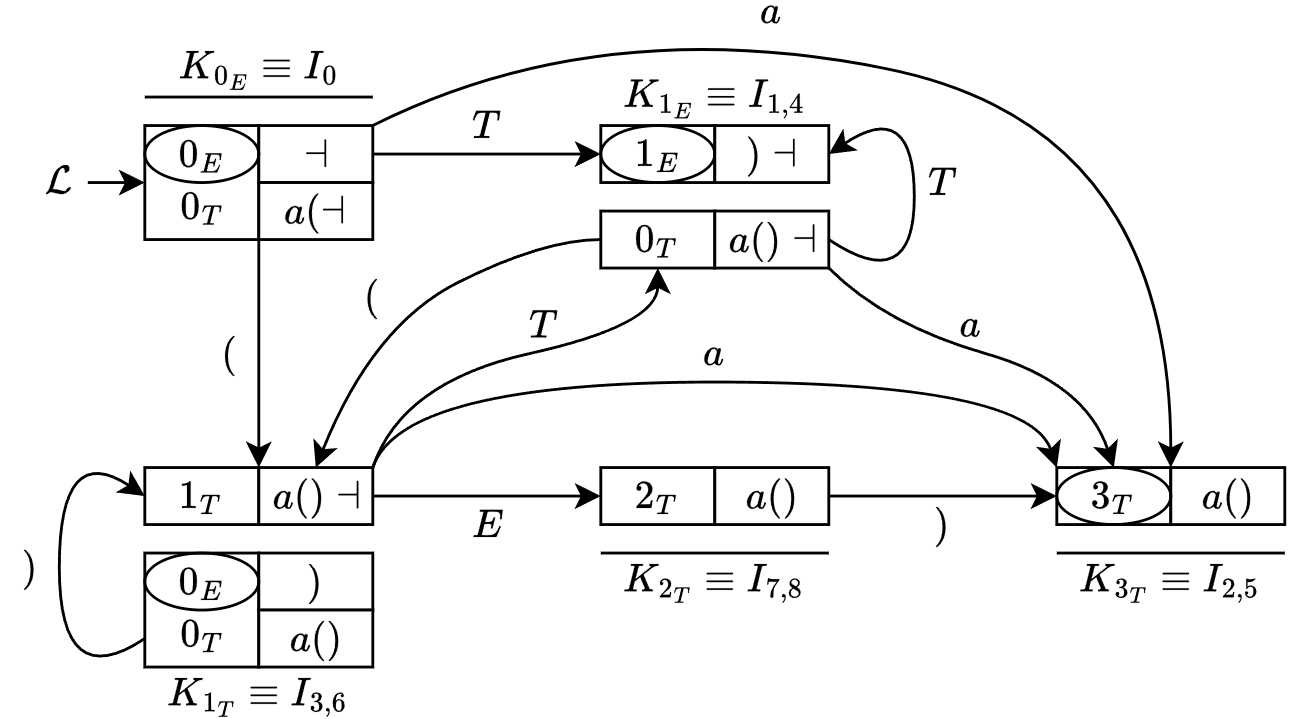
\includegraphics[width=0.6\linewidth]{images/pil1.png}
    \end{figure}
\end{example}

\subsection{Parser control-flow graph}
The Parser Control-Flow Graph (PCFG) serves as the control unit for the ELL(1) syntax analyzer. 
In this structure, prospect sets are exclusively incorporated into the final states, guiding the decision to either terminate the machine or proceed with additional moves.
Dashed call arcs are labeled with a guide set, representing the set of anticipated characters in the input following the machine call. 
This guide set enables choices such as:
\begin{itemize}
    \item Executing one call move. 
    \item Scanning a terminal symbol. 
    \item Executing one of two or more call moves. 
    \item Exiting the machine (if final state).
\end{itemize}
\begin{example}
    Considering the pilot from the previous example, the corresponding Parser Control-Flow Graph is illustrated below:
    \begin{figure}[H]
        \centering
        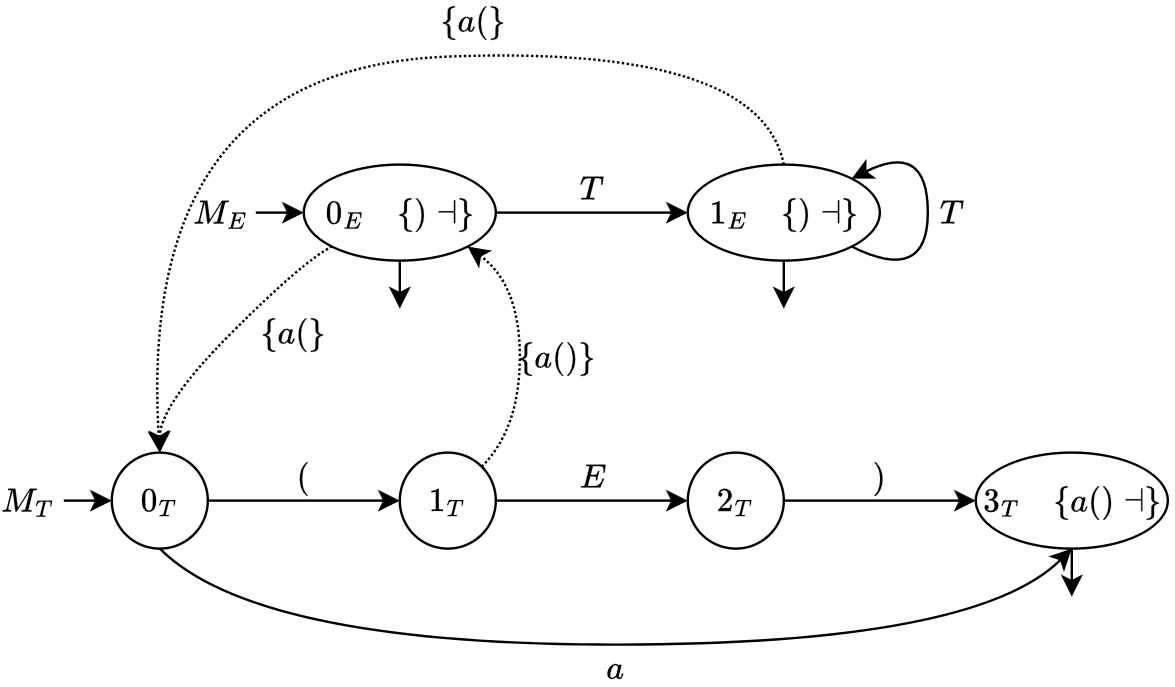
\includegraphics[width=0.6\linewidth]{images/pcfg.png}
    \end{figure}
\end{example}

The inclusion of the character $b$ is in the guide set, denoted as $b \in \textnormal{Gui}(q_A \dashrightarrow 0_{A_1})$, if one of the following properties holds:  
\begin{itemize}
    \item $b \in \textnormal{Ini}(L(0_{A_1}))$. 
    \item $A_1$ is nullable and $b \in \textnormal{Ini}(L(r_A))$. 
    \item $A_1$ and $L(r_A)$ are both nullable and $b \in \pi_{r_A}$.
    \item Exists in $\mathcal{F}$ a call arc $0_{A_1} \overset{\gamma_2}{\dashrightarrow} 0_{A_2}$ and $b \in \gamma_2$. 
\end{itemize}
The guide sets of call arcs departing from the same state must be mutually exclusive and disjoint from all scan arcs originating from the same state.

Within a PCFG, nearly all arcs (excluding non-terminal shifts) are interpreted as conditional instructions:
\begin{itemize}
    \item Terminal arcs $p \overset{a}{\rightarrow} q$ run if an only if the current character $cc=a$. 
    \item Call arcs $q_A \rightarrow 0_B$ run if an only if the current character is $cc \in \textnormal{Gui}(q_A \rightarrow 0_B)$. 
    \item Exit arcs (darts) $f_A \rightarrow$ from a state with an item $\left\langle f_A, \pi \right\rangle$ run if and only if the current character is $cc \in \pi$. 
    \item The non-terminal arcs $p \overset{a}{\rightarrow} q$ are interpreted as (unconditioned) return instructions from a machine. 
\end{itemize}
\begin{property}
    If the guide sets are disjoint, then the condition for ELL(1) is satisfied. 
\end{property}

\subsection{Algorithm}
The stack elements in the ELL syntax analyzer represent the states of the Parser Control-Flow Graph (PCFG).
Initialization of the stack involves the insertion of the element $\left\langle 0_E \right\rangle$. 
Assuming $\left\langle q_A \right\rangle$ is at the stack's top (indicating that machine $M$ is active and in state $q_A$), the ELL syntax analyzer operates through four types of moves:
\begin{itemize}
    \item \textit{Scan move}: if the shift arc $q_A \overset{cc}{\rightarrow}r_A$ exists, the analyzer performs a scan move by advancing to the next token and replacing the stack top with $\left\langle r_A \right\rangle$ (the active machine remains unchanged).
    \item \textit{Call move}: if the presence of a call arc $q_A \overset{\gamma}{\dashrightarrow} 0_B$ where  $cc \in \gamma$, and with the corresponding non-terminal shift arc $q_A \overset{B}{\rightarrow}r_A$, the analyzer executes a call move. 
        This involves popping the stack, pushing the element $\left\langle r_A \right\rangle$, and pushing the element $\left\langle 0_B \right\rangle$.
    \item \textit{Return move}: if $q_A$ is a final state, and the token $cc$ is in the prospect set associated with $q_A$, the analyzer performs a return move by popping the stack.
    \item \textit{Recognition move}: if $M_A$ is the axiom machine, $q_A$ is a final state, and $cc =\dashv$, the analyzer accepts the input and halts.
\end{itemize}
In any other scenario, the analyzer stops and rejects the input string.

\subsection{Parser implementation by means of recursive procedures}
This implementation transforms the machine into a procedure devoid of parameters, resulting in a unique procedure for each nonterminal. 
Consequently, a call move translates into a procedure call, a scan move transforms into a call to the next procedure, and a return move becomes a return from the procedure. 
The Parser Control Flow Graph now serves as the control graph for these procedures.
To determine which move to execute, the guide sets and prospect sets are employed. 
The analysis initiates by invoking the axiomatic procedure. 
In summary:
\begin{itemize}
    \item A call move corresponds to a procedure call.
    \item A scan move is akin to calling the next procedure.
    \item A return move translates into returning from the procedure.
\end{itemize} 
The selection of the move to execute is guided by the information in the guide sets and prospect sets. 
The entire process begins by invoking the axiomatic procedure.

\subsection{Direct construction of the parser control-flow graph}
The construction of the Parser Control-Flow Graph (PCFG) is achievable without the necessity of building the complete ELR pilot graph. 
This is accomplished by introducing call arcs to the machine net and annotating the net with prospect and guide sets.

To formulate the prospect set, a distinction is made between initial states and other states. 
For initial states $0_A$, the prospect set is defined as follows:
\[\pi_{0_A}:=\pi_{0_A} \cup \bigcup_{q_i \overset{A}{\rightarrow} r_i}\left( \textnormal{Ini}(L(r_i)) \cup \textnormal{ if Null}(L(r_i)) \textnormal{ then } \pi_{q_i} \textnormal{ else } \varnothing \right)\]
For every non-initial state $q$, the prospect set is defined as:
\[\pi_q:=\bigcup_{p_i \overset{X_i}{\rightarrow}q}\pi_{p_i}\]

To construct the guide set, the following iterative formula is applied:
\[\textnormal{Gui}(q_A \dashrightarrow 0_{A_1}):=\bigcup
\begin{cases}
    \textnormal{Ini}(L(A_1)) \\
    \textnormal{If Null}(A_1) \textnormal{ then Ini}(L(r_A)) \textnormal{ else } \varnothing \\
    \textnormal{If Null}(A_1) \land \textnormal{Null}(L(r_A)) \textnormal{ then Ini}(\pi_(r_A)) \textnormal{ else } \varnothing \\
    \bigcup_{0_{A_1} \dashrightarrow 0_{B_i}}\textnormal{Gui}(0_{A_1} \dashrightarrow 0_{B_i})
\end{cases}\]
Additionally, for the final darts and the terminal shift arcs, the guide sets are defined as:
\[\textnormal{Gui}(f_A \rightarrow):=\pi_{f_A}\]
\[\textnormal{Gui}(q_A \overset{a}{\rightarrow}r_A):=\{a\}\]

\subsection{Modification of grammar not in ELL(1)}
In the event that the ELL(1) condition is not met, one strategy involves attempting to modify the grammar to conform to the ELL(1) type. 
However, this process may be time-consuming and demanding.

Alternatively, an approach is to employ a longer look-ahead. The analyzer examines a sequence of $k > 1$ consecutive characters in the input. 
If the guide sets of length $k$ on alternative moves are disjoint, then an ELL(k) analysis becomes feasible.
This alternative approach provides a way to accommodate more complex grammars by considering a greater number of characters in the look-ahead, potentially resolving conflicts that arise with the ELL(1) condition.